\chapter{SYSTEM DESIGN}

\justify
This chapter outlines the detailed system design of our 5G SA CU-DU split simulation. We will cover the logical interface bindings, diagram the F1 handover message sequences, map out the UE state machine, and document the complete configuration parameter schema used across all network nodes.

\section{Interface Architecture}
\justify
Our testbed implements three logical interfaces standardized by 3GPP, linking the core network, centralized radio controller, distributed radios, and user terminals:
\begin{itemize}[leftmargin=*]
    \item \textbf{NG Interface (CU $\leftrightarrow$ Core):}
    \begin{itemize}
        \item \textbf{NG-C (Control Plane):} Uses NGAP (Next Generation Application Protocol) over SCTP. The CU at \texttt{127.0.0.11} connects to the AMF at \texttt{127.0.0.5}. Handles NAS transport, UE context management, and PDU session resource setup.
        \item \textbf{NG-U (User Plane):} Uses GTP-U (GPRS Tunneling Protocol - User) over UDP port 2152. The CU forwards encapsulated user data to/from the UPF at \texttt{127.0.0.20}.
    \end{itemize}
    
    \item \textbf{F1 Interface (CU $\leftrightarrow$ DUs):}
    \begin{itemize}
        \item \textbf{F1-C (Control Plane):} Uses F1AP (F1 Application Protocol) over SCTP on port 2153. Carries UE Context Setup/Modification/Release messages, DL/UL RRC Message Transfers, and paging.
        \item \textbf{F1-U (User Plane):} Uses GTP-U over UDP on port 2153. Carries user-plane PDUs between CU-PDCP and DU-RLC.
    \end{itemize}
    
    \item \textbf{Uu Interface (DUs $\leftrightarrow$ UE):} The air interface, emulated by the OAI RFsimulator. DU0 uses port 4043 (serving) and DU1 uses port 4044 (target). IQ samples are encapsulated in UDP packets over the loopback interface.
\end{itemize}

\begin{figure}[H]
\centering
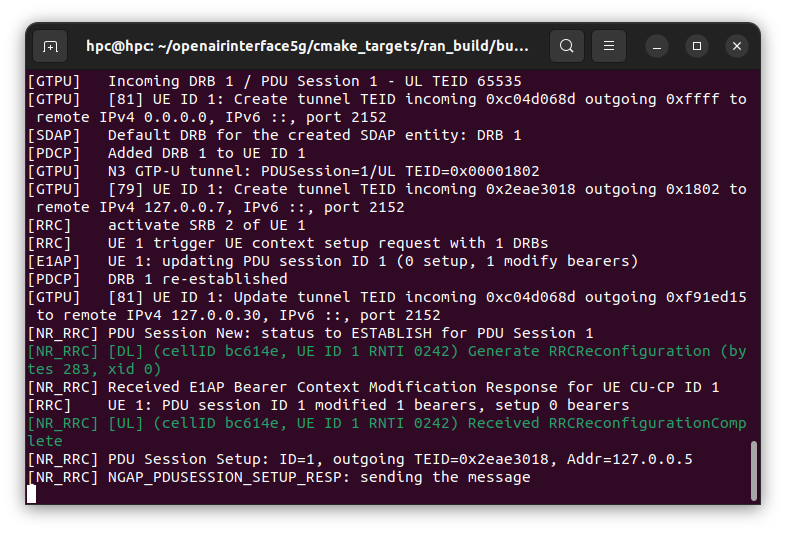
\includegraphics[width=0.85\textwidth]{images/pdu-session-establishment-cu-terminal.png}
\caption{CU console showing PDU session establishment and F1 interface activation}
\label{fig:pdu_session}
\end{figure}


\section{F1 Handover Protocol Sequence}
\justify
To execute our intra-CU handover, the system orchestrates a precise sequence of F1AP control messages and RRC reconfigurations across the network nodes. The complete message flow is mapped out in Figure~\ref{fig:ho_flow} and detailed in Table~\ref{tab:ho_steps}.

\begin{figure}[H]
\centering
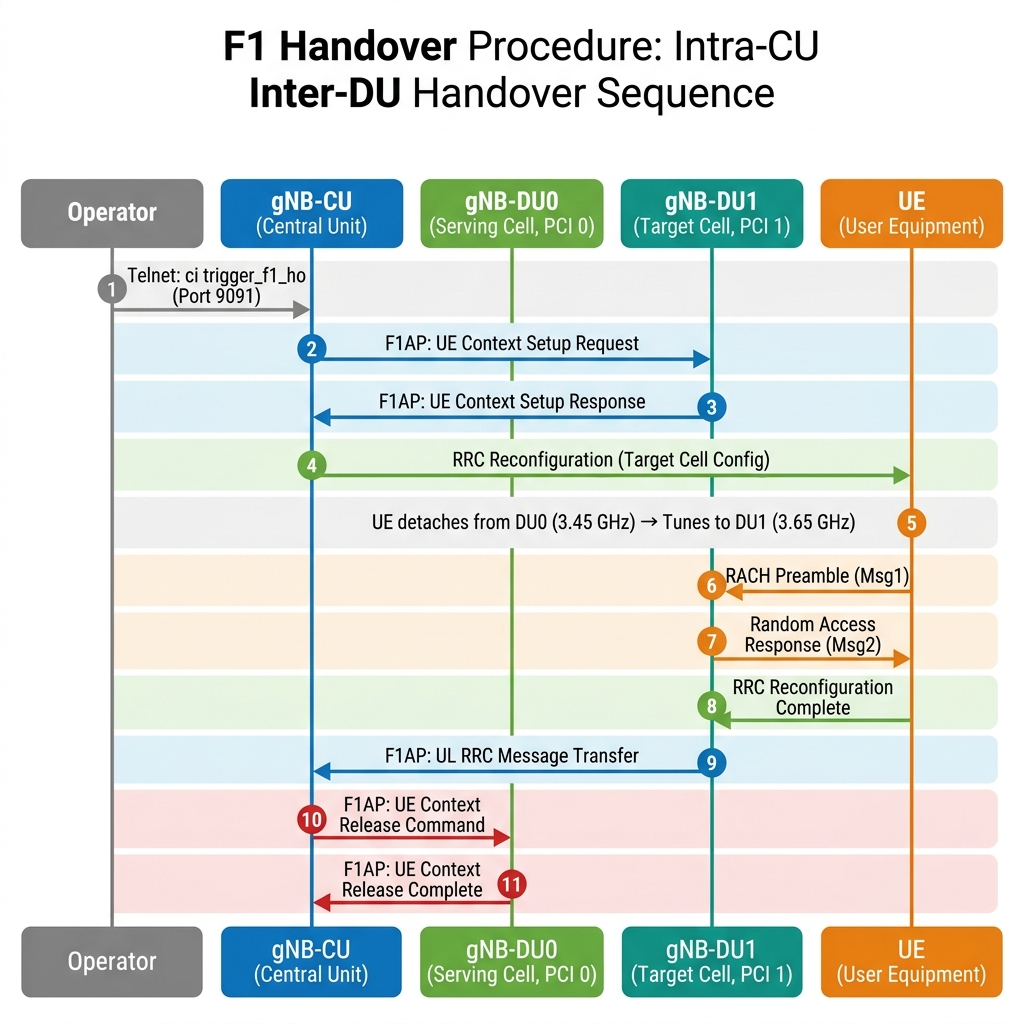
\includegraphics[width=0.95\textwidth]{images/handover_flow.png}
\caption{F1 Handover Procedure: Complete message sequence between Operator, CU, DU0, DU1, and UE}
\label{fig:ho_flow}
\end{figure}

Figure \ref{fig:ho_flow} illustrates the complete handover flow. The detailed steps are documented in Table \ref{tab:ho_steps}.

\begin{table}[H]
\centering
\small
\begin{tabular}{|c|l|c|c|p{6.5cm}|}
\hline
\textbf{Step} & \textbf{Message} & \textbf{From} & \textbf{To} & \textbf{Description} \\ \hline
1 & Telnet Command & Operator & CU & \texttt{ci trigger\_f1\_ho} via port 9091 \\ \hline
2 & UE Context Setup Req & CU & DU1 & F1AP: Prepare target cell resources \\ \hline
3 & UE Context Setup Resp & DU1 & CU & F1AP: C-RNTI and RACH config allocated \\ \hline
4 & RRC Reconfiguration & CU & UE & Via DU0: Target cell group config \\ \hline
5 & Frequency Switch & UE & -- & Detach from 3.45~GHz, tune to 3.65~GHz \\ \hline
6 & RACH Preamble (Msg1) & UE & DU1 & Random access on target cell \\ \hline
7 & RAR (Msg2) & DU1 & UE & Timing advance + UL grant \\ \hline
8 & RRC Reconfig Complete & UE & DU1 & Handover confirmation \\ \hline
9 & UL RRC Msg Transfer & DU1 & CU & F1AP: Forward RRC Complete to CU \\ \hline
10 & UE Context Release Cmd & CU & DU0 & F1AP: Release old context \\ \hline
11 & UE Context Release Cpl & DU0 & CU & F1AP: Confirm resource deallocation \\ \hline
\end{tabular}
\caption{F1 Handover Execution Steps}
\label{tab:ho_steps}
\end{table}


\section{UE State Transition Diagram}
\justify
During the F1 handover process, the User Equipment transitions through a sequence of internal state changes as it shifts its physical radio bindings from DU0 to DU1:

\begin{enumerate}[leftmargin=*]
    \item \textbf{RRC\_CONNECTED\_DU0:} UE is fully connected to DU0 at 3.45~GHz (rfsimulator port 4043). Active PDU session with IP from \texttt{10.45.0.0/16} subnet. User-plane data flows through DU0 $\rightarrow$ CU $\rightarrow$ UPF $\rightarrow$ DN.
    
    \item \textbf{RRC\_RECONFIGURING:} Upon receiving the \texttt{RRCReconfiguration} message containing the target CellGroupConfig, the UE suspends transmission on DU0, stores the serving cell context, and prepares the target cell configuration.
    
    \item \textbf{RACH\_ACTIVE\_DU1:} The UE tunes its RF interface to DU1's frequency (3.65~GHz, rfsimulator port 4044) and transmits the dedicated RACH preamble (Msg1). It then listens for the Random Access Response (RAR/Msg2) containing timing advance and uplink scheduling grant.
    
    \item \textbf{RRC\_CONNECTED\_DU1:} Upon successful RACH, the UE applies timing adjustments, sends \texttt{RRCReconfigurationComplete}, and resumes user-plane data transmission via DU1. The PDU session remains active and uninterrupted --- only the radio path has changed.
\end{enumerate}


\section{Configuration Parameters Schema}
\justify
To ensure our simulation results are reproducible and to provide a quick reference for reviewers, we compiled the complete configuration schema for the CU, DUs, and UE processes into the master parameter mapping in Table~\ref{tab:params}.

\begin{longtable}{|p{4cm}|c|c|c|c|}
\hline
\textbf{Parameter} & \textbf{gNB-CU} & \textbf{DU0} & \textbf{DU1} & \textbf{UE} \\ \hline
\endfirsthead
\hline
\textbf{Parameter} & \textbf{gNB-CU} & \textbf{DU0} & \textbf{DU1} & \textbf{UE} \\ \hline
\endhead
\hline
\endfoot

\multicolumn{5}{|l|}{\textbf{Network Identity}} \\ \hline
gNB ID & 0xe00 & 0xe00 & 0xe00 & -- \\ \hline
gNB DU ID & -- & 0xe03 & 0xe04 & -- \\ \hline
PLMN (MCC/MNC) & 001/01 & 001/01 & 001/01 & 001/01 \\ \hline
Tracking Area Code & 7 & 7 & 7 & -- \\ \hline
S-NSSAI (SST) & 1 & 1 & 1 & 1 \\ \hline

\multicolumn{5}{|l|}{\textbf{Cell Identity \& Radio}} \\ \hline
NR Cell ID & 12345678L & 12345678L & 22222222L & -- \\ \hline
Physical Cell ID & -- & 0 & 1 & -- \\ \hline
Frequency Band & -- & n78 (TDD) & n78 (TDD) & n78 \\ \hline
SSB Freq (ARFCN) & -- & 630048 & 643296 & both \\ \hline
Point A (ARFCN) & -- & 628776 & 642024 & -- \\ \hline
Center Freq (Hz) & -- & 3,450,720,000 & 3,649,440,000 & both \\ \hline
SCS / Numerology & -- & 30 kHz / $\mu$=1 & 30 kHz / $\mu$=1 & $\mu$=1 \\ \hline
Bandwidth (PRBs) & -- & 106 & 106 & 106 \\ \hline

\multicolumn{5}{|l|}{\textbf{Interface \& Transport}} \\ \hline
F1 IP Address & 127.0.0.11 & 127.0.0.29 & 127.0.0.30 & -- \\ \hline
F1 Port (SCTP/GTP) & 2153 & 2153 & 2153 & -- \\ \hline
AMF IP Address & 127.0.0.5 & -- & -- & -- \\ \hline
RFsim Port & -- & 4043 & 4044 & 4043/4044 \\ \hline
Telnet Port & 9091 & -- & -- & -- \\ \hline

\multicolumn{5}{|l|}{\textbf{TDD Frame Structure}} \\ \hline
DL/UL Periodicity & -- & 5 ms & 5 ms & -- \\ \hline
DL Slots / Symbols & -- & 7 / 6 & 7 / 6 & -- \\ \hline
UL Slots / Symbols & -- & 2 / 4 & 2 / 4 & -- \\ \hline

\multicolumn{5}{|l|}{\textbf{RACH Configuration}} \\ \hline
PRACH Config Index & -- & 98 & 98 & -- \\ \hline
Root Seq Index & -- & 1 (len 139) & 1 (len 139) & -- \\ \hline
Preamble Target Pwr & -- & $-96$ dBm & $-96$ dBm & -- \\ \hline
SSB Periodicity & -- & 20 ms & 20 ms & -- \\ \hline

\multicolumn{5}{|l|}{\textbf{Security}} \\ \hline
Ciphering Alg. & NEA0 & -- & -- & -- \\ \hline
Integrity Alg. & NIA2 & -- & -- & -- \\ \hline

\multicolumn{5}{|l|}{\textbf{UE Subscriber}} \\ \hline
IMSI & -- & -- & -- & 001010000007487 \\ \hline
DNN & -- & -- & -- & internet \\ \hline
Dual-RU Count & -- & -- & -- & 2 \\ \hline
Max RX Gain & -- & 114 dB & 114 dB & 114 dB \\ \hline

\multicolumn{5}{|l|}{\textbf{Measurement Events}} \\ \hline
A2 Threshold & \multicolumn{4}{c|}{60 (RSRP)} \\ \hline
A3 Offset (PCI 1) & \multicolumn{4}{c|}{10 dB, Hysteresis: 0, TTT: 1} \\ \hline
A3 Offset (PCI 0) & \multicolumn{4}{c|}{5 dB, Hysteresis: 1, TTT: 2} \\ \hline
Channel Model & \multicolumn{4}{c|}{AWGN} \\ \hline

\caption{Master Configuration Parameters Table}
\label{tab:params}
\end{longtable}
